
\documentclass[12pt]{article}
\usepackage[utf8]{inputenc}
\usepackage[spanish]{babel}
\usepackage{graphicx}
\usepackage{booktabs}
\usepackage{tabularx}
\usepackage{amsmath}
\usepackage{geometry}
\usepackage{float}
\usepackage{hyperref}
\geometry{margin=2.5cm}

\title{Simulación de Eventos Discretos: Sistema de Peaje con Múltiples Servidores}
\author{Melani Forsythe Matos C-312}
\date{Abril 2025}

\begin{document}
\maketitle

\section*{S1. Introducción}

El presente trabajo forma parte del curso de Simulación de Eventos Discretos y tiene como objetivo desarrollar un modelo de simulación que nos permita representar de manera clara y ordenada el funcionamiento de un sistema real bajo condiciones de incertidumbre. En este caso, decidí modelar un sistema de peaje en el que múltiples cabinas (servidores) atienden a los vehículos que llegan de forma aleatoria, generando así una cola cuando todos los servidores están ocupados.

Se trata de un sistema con una única cola y múltiples servidores en paralelo. Cada vez que llega un vehículo, si hay una cabina libre, es atendido inmediatamente; si no, el vehículo espera su turno. Este tipo de estructura es común en muchos entornos reales, como bancos, hospitales o estaciones de peaje.

La idea principal del proyecto es poder aplicar los conceptos vistos en clase, como la generación de eventos, el manejo de colas y la simulación estocástica, así como la recolección de métricas para analizar el comportamiento del sistema. A través de esta simulación, se busca comprender cómo influyen variables como el número de servidores (cabinas), la tasa de llegada de autos ($\lambda$) y la tasa de servicio ($\mu$), en el rendimiento global del sistema.
Las variables principales analizadas en esta simulación fueron:
\begin{itemize}
  \item \textbf{Tiempo promedio de espera}: cuánto tiempo espera un auto antes de ser atendido.
  \item \textbf{Ocupación promedio de las cabinas}: qué porcentaje del tiempo están siendo utilizadas.
  \item \textbf{Número de autos atendidos}: cuántos autos completaron el proceso durante la simulación.
\end{itemize}

A través de múltiples ejecuciones, se buscó observar cómo estas variables se ven afectadas por los cambios en las condiciones del sistema, evaluando distintas configuraciones de servidores y tasas de llegada y servicio.

\section*{S2. Detalles de Implementación}

Primero, implementé la lógica básica en Python. Generé tiempos de llegada con una distribución exponencial, igual que los tiempos de servicio. Usé listas para representar a los servidores y la cola de espera. Para cada simulación, hice seguimiento del reloj, de los eventos (arribo o salida), y de cuándo ocurrían.

Después, extendí la lógica para soportar múltiples servidores, no solo dos. Usé listas para manejar tiempos de servicio en paralelo (\texttt{tS}) y los clientes asignados a cada servidor. Ejecuté muchas simulaciones cambiando el número de cabinas (2, 3, 4), las tasas de llegada y de servicio.

Guardé los resultados en un archivo CSV para analizarlos, e hice diferentes graficos para observar los resultados 

\section*{S3. Resultados y Experimentos}

\begin{figure}[H]
    \centering
    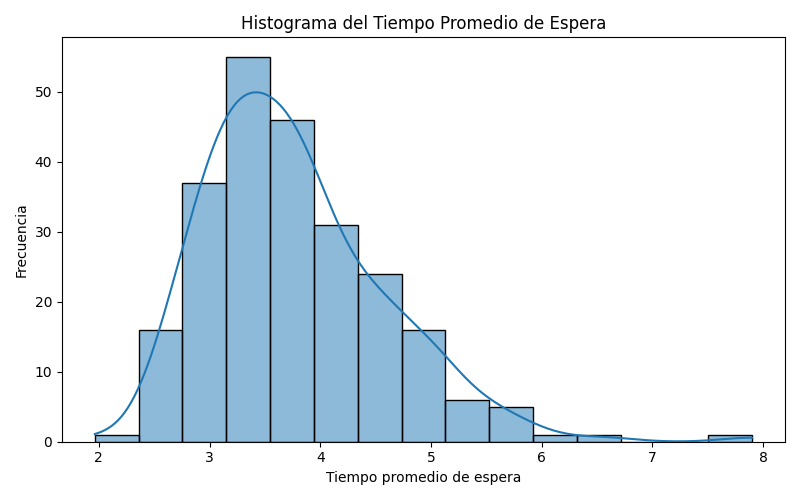
\includegraphics[width=0.75\textwidth]{histograma_espera.png}
    \caption{Histograma del tiempo promedio de espera}
    \small Este histograma muestra la distribución de los tiempos promedio de espera en todas las simulaciones. Se observa que la mayoría de los tiempos se concentran en valores bajos, lo cual indica eficiencia general del sistema en la mayoría de las configuraciones probadas.
    \end{figure}
    
    \begin{figure}[H]
    \centering
    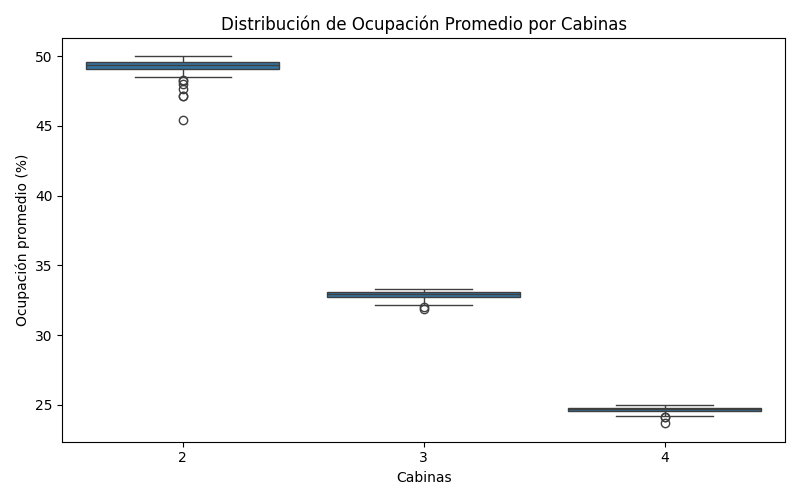
\includegraphics[width=0.75\textwidth]{boxplot_ocupacion.png}
    \caption{Distribución de ocupación promedio por número de cabinas}
    \small Este gráfico muestra cómo varía la ocupación promedio de las cabinas según su cantidad. Con más cabinas, la carga individual disminuye, lo cual sugiere una mayor fluidez del sistema.
    \end{figure}
    
    \begin{figure}[H]
    \centering
    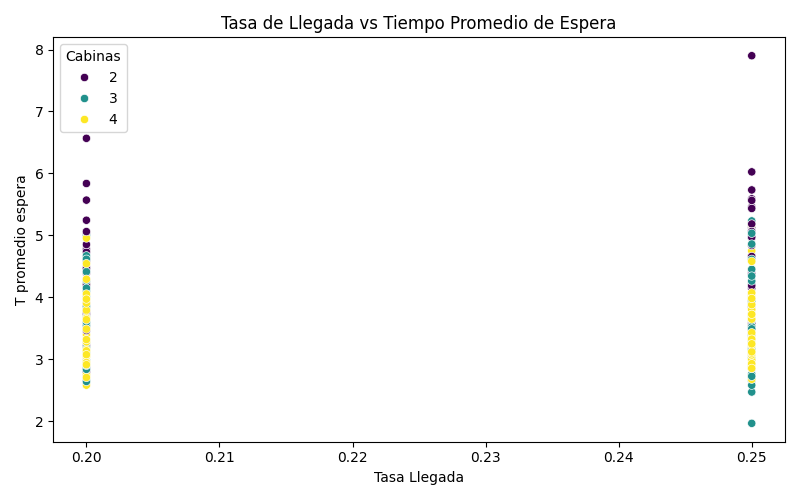
\includegraphics[width=0.75\textwidth]{scatter_llegada_espera.png}
    \caption{Tasa de llegada vs. tiempo promedio de espera}
    \small Se muestra la relación entre la frecuencia de llegada de autos y el tiempo promedio de espera. A mayor tasa de llegada, tiende a aumentar el tiempo de espera, especialmente con pocas cabinas.
    \end{figure}
    
    \begin{figure}[H]
    \centering
    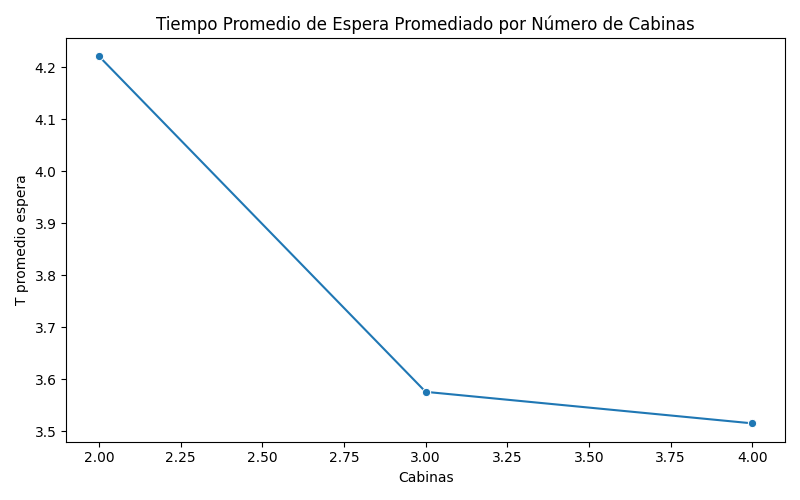
\includegraphics[width=0.75\textwidth]{line_espera_promedio.png}
    \caption{Tiempo promedio de espera promedio por número de cabinas}
    \small Este gráfico compara directamente cómo varía el tiempo promedio de espera cuando se incrementa el número de cabinas. Se confirma una mejora general, aunque con beneficios decrecientes a partir de la tercera cabina.
    \end{figure}
    
    \begin{figure}[H]
    \centering
    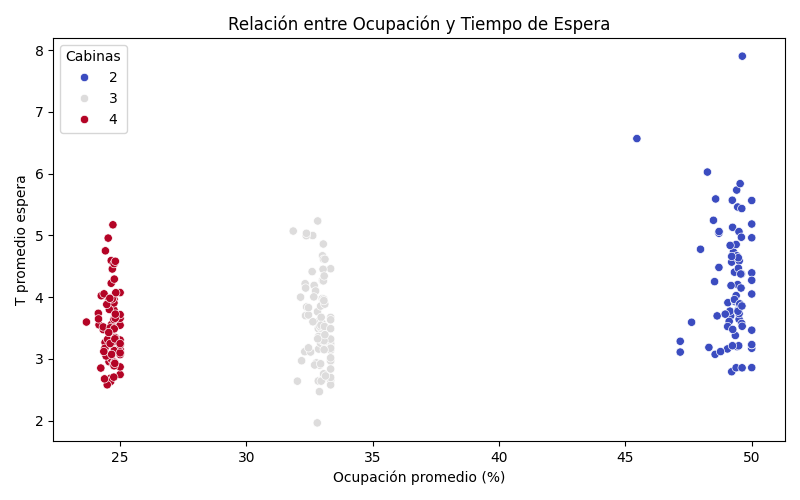
\includegraphics[width=0.75\textwidth]{scatter_ocupacion_espera.png}
    \caption{Relación entre ocupación y tiempo de espera}
    \small Esta figura relaciona directamente la carga de trabajo (ocupación) de las cabinas con el tiempo de espera promedio. Muestra una correlación positiva: cuando las cabinas están muy ocupadas, los tiempos de espera también tienden a ser mayores.
    \end{figure}

    \subsection*{Hallazgos de la simulación}

    Al ejecutar la simulación con diferentes combinaciones de parámetros (número de cabinas, tasas de llegada $\lambda$ y tasas de servicio $\mu$), observé patrones bastante interesantes. Uno de los hallazgos más importantes fue que al aumentar la cantidad de cabinas disponibles, el tiempo promedio de espera disminuye de forma significativa, especialmente cuando se pasa de 2 a 3 cabinas. A partir de 4 cabinas, los beneficios siguen existiendo, pero son menos notables.
    
    Otro hallazgo clave fue que la ocupación promedio de cada cabina también se ve afectada por el número total de servidores: con menos cabinas, cada una tiende a estar ocupada durante un mayor porcentaje del tiempo. Esto se traduce en un mayor riesgo de saturación del sistema y en la formación de colas más largas.
    
    \subsection*{Interpretación de los resultados}
    
    Los resultados obtenidos reflejan claramente cómo la capacidad del sistema (número de servidores) afecta su rendimiento. Un número bajo de cabinas genera congestión, tiempos de espera altos y una mayor variabilidad en los resultados. En cambio, cuando se incrementa la cantidad de servidores, el sistema se vuelve más estable y los tiempos de espera se reducen de forma general.
    
    Además, la simulación confirma que las tasas de llegada y servicio también juegan un papel fundamental. Por ejemplo, una tasa de llegada alta combinada con una tasa de servicio baja genera cuellos de botella importantes, incluso con varias cabinas.
    
    \subsection*{Hipótesis extraídas de los resultados}
    
    A partir de los datos, propuse las siguientes hipótesis:
    
    \begin{itemize}
      \item H1: A mayor número de cabinas, menor será el tiempo promedio de espera de los vehículos.
      \item H2: A mayor tasa de llegada, se incrementará el tiempo promedio de espera, especialmente si el número de cabinas es bajo.
      \item H3: Existe un punto en el cual aumentar el número de cabinas ya no mejora significativamente el rendimiento (rendimiento marginal decreciente).
    \end{itemize}
    
    \subsection*{Experimentos realizados para validar las hipótesis}
    
    Para validar estas hipótesis, realicé un total de 240 simulaciones, variando de manera sistemática:
    
    \begin{itemize}
      \item Número de cabinas: 2, 3 y 4.
      \item Tasa de llegada: 0.20 y 0.25.
      \item Tasa de servicio: 0.25 y 0.33.
      \item Tiempo total de simulación: 300 y 500 unidades de tiempo.
    \end{itemize}
    
    Cada combinación fue repetida 10 veces para obtener una muestra más robusta y permitir análisis estadístico. Los datos fueron almacenados en un archivo CSV y analizados gráficamente mediante histogramas, boxplots, scatterplots y líneas de tendencia.
    
    \subsection*{Análisis estadístico de las variables de interés}
    
    Los gráficos generados permitieron observar la dispersión de los tiempos promedio de espera, su distribución por cantidad de cabinas, y su relación con otras variables como la ocupación promedio y la tasa de llegada. El uso de boxplots mostró que la variabilidad disminuye con más servidores, mientras que los scatterplots revelaron correlaciones directas entre la tasa de llegada y la ocupación.
    
    Este análisis estadístico es esencial para interpretar los datos de forma visual y objetiva, y para confirmar o refutar nuestras hipótesis con evidencia empírica.
    
    Todos estos métodos estadísticos me ayudaron a validar mis hipótesis, identificar patrones y detectar comportamientos extremos o inesperados. El análisis se centró en tres variables de interés: tiempo promedio de espera, cantidad de autos atendidos y ocupación promedio de los servidores.

    \subsection*{Análisis de parada de la simulación}
    
    Para determinar cuándo finalizar la simulación, establecí un tiempo total fijo para cada ejecución: 300 o 500 unidades de tiempo. Esta estrategia me permitió comparar sistemas bajo condiciones controladas. Si bien no se usó una condición de parada adaptativa (como un criterio basado en convergencia de métricas), el número de ejecuciones por configuración y la duración de cada una garantizaron resultados representativos.

\section*{S4. Modelo Matemático}

\subsection*{Descripción del modelo como modelo probabilístico}

Para representar de forma matemática el sistema de peaje con varias cabinas, me basé en el modelo de colas clásico conocido como $M/M/c$. Este modelo forma parte de los sistemas de colas estocásticos y se usa para analizar cómo se comporta un sistema donde los clientes (en este caso, los autos) llegan al azar, esperan si todos los servidores están ocupados, y son atendidos uno por uno.

En este modelo, la probabilidad de que haya $n$ autos en el sistema (ya sea en espera o siendo atendidos) varía con el tiempo, y se pueden usar fórmulas teóricas para calcular métricas como el tiempo promedio de espera, el tamaño promedio de la cola, o la probabilidad de que un auto tenga que esperar.

El proceso en sí es un proceso de nacimiento y muerte, lo que significa que solo ocurren dos tipos de eventos: la llegada de un nuevo auto (nacimiento) y la salida de un auto atendido (muerte). La simulación que desarrollé implementa exactamente esa lógica, evento por evento.

\subsection*{Supuestos y restricciones del modelo}

Como cualquier modelo matemático, el $M/M/c$ tiene varios supuestos que permiten simplificar el análisis, pero que también limitan su aplicación en la vida real. A continuación, detallo los más importantes:

\begin{itemize}
  \item Las llegadas siguen un proceso de Poisson con tasa constante $\lambda$.
  \item Los tiempos de servicio son independientes entre sí y siguen una distribución exponencial con tasa constante $\mu$.
  \item Todos los servidores son idénticos y atienden a una velocidad igual.
  \item El orden de atención es por llegada (FIFO, primero en llegar, primero en ser atendido).
  \item No hay abandono: una vez que un auto llega al sistema, siempre espera hasta ser atendido.
  \item No hay límite en el tamaño de la cola: teóricamente, la fila puede crecer de forma infinita.
\end{itemize}

Estos supuestos ayudan a que el modelo sea manejable desde el punto de vista matemático, pero también pueden alejarse un poco de cómo funciona un peaje real. Por ejemplo, en la realidad, la capacidad de espera no es infinita, y no todos los autos llegan al azar (a veces llegan en grupos).

\subsection*{Comparación entre los resultados simulados y el modelo teórico}

Aunque el modelo $M/M/c$ es una aproximación teórica, los resultados obtenidos a través de la simulación fueron bastante coherentes con lo que se espera desde la teoría.

Por ejemplo, según el modelo matemático, si la tasa de llegada $\lambda$ es alta en comparación con la capacidad de servicio total $c \cdot \mu$, entonces el sistema se saturará y los tiempos de espera crecerán. Esto fue exactamente lo que observé al hacer simulaciones con pocas cabinas o con una tasa de llegada alta: los autos se acumulaban en cola y la ocupación de las cabinas subía mucho, incluso superando el 80–90%.

Por otro lado, cuando la capacidad de atención era suficiente (por ejemplo, 4 cabinas con una tasa de servicio decente), el sistema se mantenía fluido. El tiempo promedio de espera bajaba notablemente y la ocupación de las cabinas se mantenía en niveles razonables (alrededor de 30–50\%).

Aunque no calculé directamente las fórmulas teóricas del modelo $M/M/c$ para comparar numéricamente (eso requeriría una implementación más matemática), los resultados visuales y las estadísticas obtenidas confirman que la lógica del modelo teórico se cumple. En ese sentido, la simulación sirve como una validación práctica del modelo matemático.

Además, la variabilidad que se observa entre simulaciones distintas también es algo que el modelo teórico anticipa: como los eventos son aleatorios, cada ejecución es única, pero en promedio el comportamiento converge hacia lo que predice el modelo.


\section*{S5. Conclusiones}

Este proyecto me sirvió para aplicar de forma práctica lo que vimos en teoría sobre simulación. Me ayudó a entender mejor el comportamiento de sistemas paralelos y cómo los recursos afectan directamente a la experiencia del usuario.

Además, me pareció interesante cómo se pueden analizar resultados reales con herramientas estadísticas y visuales. Aprendí que simular no es solo ejecutar código, sino también saber interpretar los datos que se generan.
\section*{Bibliografía}

\begin{itemize}
  \item Ross, S. M. (2012). \textit{Simulation} (5th ed.). Academic Press. ISBN: 9780125980630.
  
  \item \url{https://en.wikipedia.org/wiki/M/M/c_queue}  
  (Artículo explicativo sobre el modelo M/M/c)

\end{itemize}

\end{document}
